\documentclass{beamer}

\usetheme{CambridgeUS}

\usepackage[utf8]{inputenc}
\usepackage{datetime}
\usepackage{amsmath}
\usepackage{tikz}

\newdate{date}{09}{03}{2018}
\date{\displaydate{date}}

\tikzstyle{vertex} = [fill,shape=circle,node distance=40pt]
\tikzstyle{edge} = [fill,opacity=.5,fill opacity=.5,line cap=round, line join=round, line width=25pt]
\tikzstyle{elabel} =  [fill,shape=circle,node distance=15pt]

\pgfdeclarelayer{background}
\pgfsetlayers{background,main}

\begin{document}

\begin{frame}
\begin{itemize}
    \item $k$-anonymity Defined
    \item $k$-anonymity-test is in P
    \item 3-anonymity is NP-hard (Meyerson \& Williams)
    \item 2-anonymity is in P (Blocki \& Williams)
\end{itemize}
\end{frame}

\begin{frame}
\frametitle{$k$-anonymity Defined}
A database $V$ is a multiset of $m$-degree attribute tuples with each tuple $\in \Sigma^{m}$ where $\Sigma$ is the domain of attributes. $v[i]$ projects $i$th attribute in $v$.\\~\\

A database $V$ is $k$-anonymous iff, for all $v \in V$, there exist a subset $S \subseteq V$ of size $k$ such that, for all $s,s' \in S$, $s=s'$.\\~\\

A suppressor $t$ on a database $V$ is a mapping $V \rightarrow \{\Sigma \cup \{*\}\}^{m}$ such that, for all $v \in V$, for all $j \in \{1,...,m\}$, $t(v)[j] \in \{v[j], *\}$. $t(v)[j]$ is suppressed iff $t(v)[j] = *$.\\~\\

For a suppressor $t$ and a database $V$, $t(V) = \{t(v) : v \in V\}$. If $t(V)$ is $k$-anonymous, $t$ is called a $k$-anonymizer on $V$.
\end{frame}

\begin{frame}
\frametitle{$k$-anonymity-test is in P}
A database $V$ is $k$-anonymous iff, for all $v \in V$, there exist a subset $S \subseteq V$ of size $k$ such that, for all $s,s' \in S$, $s=s'$.\\~\\

\begin{block}{INSTANCE: $k$-anonymity-test}
Given a databse $V$ with column names $D$, is $\Pi_{Q} V$ $k$-anonymous for all $Q \subseteq D$.
\end{block}

It's in P.
\end{frame}

\begin{frame}
\frametitle{$k$-anonymity-test is in P}
\alert{(INSTANCE)} Given a databse $V$ with column names $D$, is $\Pi_{Q} V$ $k$-anonymous for all $Q \subseteq D$.\\~\\

\begin{block}{Sweeney's Lemma: remove columns can only make it k-anonymous}
For relational table $RT$ of $m$-tuples with column names $D$, if $\Pi_{H} RT$ is k-anonymous, then $\Pi_{K} RT$ is k-anonymous, for $K \subseteq H \subseteq D$.
\end{block}

\alert{Naive Algorithm}
Check the case of QI=$D$. It runs in $\mathcal{O}(n^2mk)$.\\~\\

\alert{Proof}
\begin{itemize}
    \item If it checks out: then it is k-anonymous \alert{for all possible QIs}, with Sweeney's Lemma.
    \item If it fails: then it is not k-anonymous \alert{for the QI of all attributes}.
\end{itemize}
\end{frame}

\begin{frame}
\frametitle{3-anonymity is NP-hard}
NP-hardness is shown by reduction from 3-dimensional perfect matching to 3-anonymity.\\~\\

\begin{block}{INSTANCE: 3-dimensional perfect matching (NP-complete)}
Given a simple 3-uniform hypergraph $H = (U, E)$, is there a subset of hyperedges $S \subseteq E$ of size $|U|/3$ such that each vertex of $U$ is contained in exactly one hyperedge of $S$?
\end{block}

\begin{block}{INSTANCE: 3-anonymity}
Given $V \subseteq \Sigma^{m}$ and $l \in \mathbb{N}$, is there a suppressor $t$ such that $t(V)$ is 3-anonymous and the total number of suppressions is at most $l$?
\end{block}
\end{frame}

\begin{frame}
\frametitle{3-anonymity is NP-hard}
Given a 3-uniform hypergraph $H = (U, E)$ where $U = \{u_1,...,u_n\}$ and $E = \{e_1,...,e_m\}$, construct a database $V = \{v_1,...,v_n\}$ of $m$-degree tuples such that, for all $v_i \in V$, for all $j \in \{1,...,m\}$:
$$
v_{i}[j] =
\begin{cases}
    0, & \text{if } u_i \in e_j\\
    1, & \text{otherwise}
\end{cases}
$$
\vspace*{-10pt}
\begin{columns}
\column{0.4\textwidth}
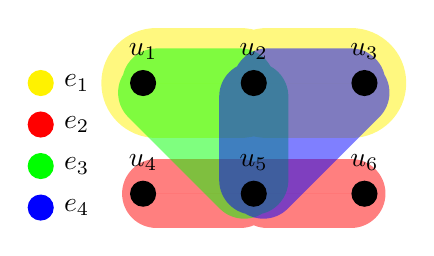
\begin{tikzpicture}
\node[vertex,label=above:            \(u_1\)] (v1) {};
\node[vertex,right of=v1,label=above:\(u_2\)] (v2) {};
\node[vertex,right of=v2,label=above:\(u_3\)] (v3) {};
\node[vertex,below of=v1,label=above:\(u_4\)] (v4) {};
\node[vertex,right of=v4,label=above:\(u_5\)] (v5) {};
\node[vertex,right of=v5,label=above:\(u_6\)] (v6) {};

\begin{pgfonlayer}{background}
\draw[edge,color=yellow,line width=40pt] (v1) -- (v2) -- (v3);
\draw[edge,color=red]    (v4) -- (v5) -- (v6);
\begin{scope}[transparency group,opacity=.5]
\draw[edge,opacity=1,color=green] (v1) -- (v2) -- (v5) -- (v1);
\fill[edge,opacity=1,color=green] (v1.center) -- (v2.center) -- (v5.center) -- (v1.center);
\end{scope}
\begin{scope}[transparency group,opacity=.5]
\draw[edge,opacity=1,color=blue] (v2) -- (v3) -- (v5) -- (v2);
\fill[edge,opacity=1,color=blue] (v2.center) -- (v3.center) -- (v5.center) -- (v2.center);
\end{scope}
\end{pgfonlayer}

\node[elabel,color=yellow,label=right:\(e_1\)]  (e1) at (-1.3,0) {};
\node[elabel,below of=e1,color=red,label=right:\(e_2\)]  (e2) {};
\node[elabel,below of=e2,color=green,label=right:\(e_3\)]  (e3) {};
\node[elabel,below of=e3,color=blue,label=right:\(e_4\)]  (e4) {};
\end{tikzpicture}

\column{0.6\textwidth}
\begin{align*}
       &  e_1 && e_2 && e_3 && e_4  &&\\
V = \{ & (0,  && 1,  && 0,  && 1),  && u_1\\
       & (0,  && 1,  && 0,  && 0),  && u_2\\
       & (0,  && 1,  && 1,  && 0),  && u_3\\
       & (1,  && 0,  && 1,  && 1),  && u_4\\
       & (1,  && 0,  && 0,  && 0),  && u_5\\
       & (1,  && 0,  && 1,  && 1)\} && u_6\\
\end{align*}
\end{columns}
\end{frame}

\begin{frame}
\frametitle{3-anonymity is NP-hard}
\alert{(Goal)} $H$ has a 3-dimensional perfect matching iff there exists a $t$ such that $t(V)$ is 3-anonymous with $l = n(m-1)$.\\
\alert{(Left to right)} Suppose $H$ has a 3-dimensional perfect matching $M$, construct a suppressor $t$ such that, for all $v_i \in V$, for all $j \in \{1,...,m\}$:
$$
t(v_{i})[j] =
\begin{cases}
    0, & \text{if } e_j \in M\\
    *, & \text{otherwise}
\end{cases}
$$
\vspace*{-15pt}
\begin{columns}
\column{0.4\textwidth}
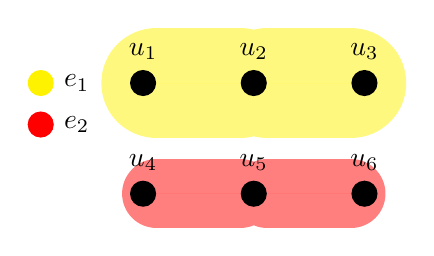
\begin{tikzpicture}
\node[vertex,label=above:            \(u_1\)] (v1) {};
\node[vertex,right of=v1,label=above:\(u_2\)] (v2) {};
\node[vertex,right of=v2,label=above:\(u_3\)] (v3) {};
\node[vertex,below of=v1,label=above:\(u_4\)] (v4) {};
\node[vertex,right of=v4,label=above:\(u_5\)] (v5) {};
\node[vertex,right of=v5,label=above:\(u_6\)] (v6) {};

\begin{pgfonlayer}{background}
\draw[edge,color=yellow,line width=40pt] (v1) -- (v2) -- (v3);
\draw[edge,color=red]    (v4) -- (v5) -- (v6);
\end{pgfonlayer}

\node[elabel,color=yellow,label=right:\(e_1\)]  (e1) at (-1.3,0) {};
\node[elabel,below of=e1,color=red,label=right:\(e_2\)]  (e2) {};
\end{tikzpicture}

\column{0.6\textwidth}
\begin{align*}
       &  e_1 && e_2 && e_3 && e_4  &&\\
V = \{ & (0,  && *,  && *,  && *),  && u_1\\
       & (0,  && *,  && *,  && *),  && u_2\\
       & (0,  && *,  && *,  && *),  && u_3\\
       & (*,  && 0,  && *,  && *),  && u_4\\
       & (*,  && 0,  && *,  && *),  && u_5\\
       & (*,  && 0,  && *,  && *)\} && u_6\\
\end{align*}
\end{columns}
\end{frame}

\begin{frame}
\frametitle{3-anonymity is NP-hard}
\alert{(Goal)} $H$ has a 3-dimensional perfect matching iff there exists a $t$ such that $t(V)$ is 3-anonymous with $l = n(m-1)$.\\
\alert{(Left to right)} Suppose $H$ has a 3-dimensional perfect matching $M$, construct a suppressor $t$ such that, for all $v_i \in V$, for all $j \in \{1,...,m\}$:
$$
t(v_{i})[j] =
\begin{cases}
    0, & \text{if } e_j \in M\\
    *, & \text{otherwise}
\end{cases}
$$

Since, for all $e_j \in M$, $|e| = 3$, there are exactly 3 identical tuples $v, v', v''$ in $t(V)$ such that $v[j] = v'[j] = v''[j] = 0$ and $v[k] = v'[k] = v''[k] = *$ for all $k \neq j$. Thus, $t(V)$ is k-anonymous. Since the matching is perfect, each tuple has exactly one $0$ and $m-1$ *s, and there are $n$ tuples. Thus, the number of suppression is exactly $n(m-1)$.
\end{frame}

\begin{frame}
\frametitle{3-anonymity is NP-hard}
\alert{(Goal)} $H$ has a 3-dimensional perfect matching iff there exists a $t$ such that $t(V)$ is 3-anonymous with $l = n(m-1)$.\\
\alert{(Right to left)} Select as hyperedges the identical tuples in $t(V)$ and we're done.\\~\\

\alert{Note} This is the case where $|\Sigma| \leq n$, but it's also NP-hard for the cases of $|\Sigma| = 3$ and $|\Sigma| = 2$; see REU Summer 2007 slides for an overview.
\end{frame}

\begin{frame}
\frametitle{2-anonymity is in P}
Reduction to polynomial time "Simplex Matching" algorithm.
\end{frame}

\end{document}
